\chapter{Formfactors}

\begin{itemize}
\item Parallelepiped
\item Pyramid
\item Cylinder
\item Cone
\item Prism3
\item Tethraedron
\item Prism6
\item Cone6
\item Sphere, \SecRef{Sphere} 
\item Cybooctaedron
\item Facetted sphere  
\item Full Sphere, \SecRef{FullSphere} 
\item Full spheroid 
\item Box
\item Anisotropic pyramid
\item Ellipsoid
\item Anisotropic hemi-spheroid
\item Spheroid
\end{itemize}

\newpage
\section{Formfactor Sphere}\SecLabel{Sphere}
%\begin{lstlisting}[language=python, style=eclipseboxed,name=ffsphere,nolol]
%from libBornAgainCore import * 
%sphere_ff = FormFactorSphere(5*nanometer, 5*nanometer)
%\end{lstlisting}
%\par
%~
%\par
Formfactor sphere is represented as a cut-off sphere with height $H$ and radius $R$. 
\begin{figure}[ht]
\begin{center}
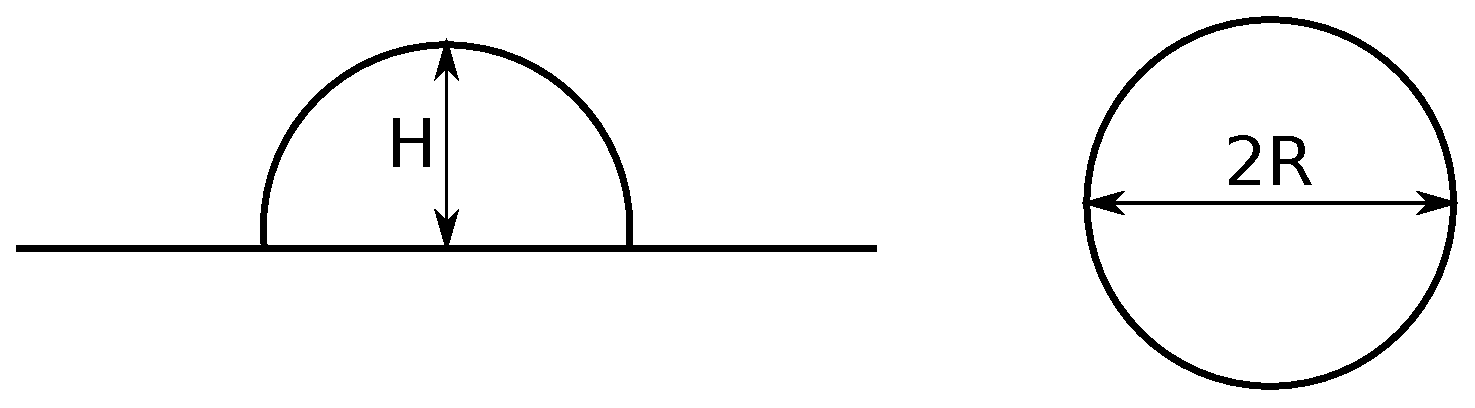
\includegraphics[width=0.6\columnwidth]{Figures/sphere}
\caption{Sketch of the formfactor sphere. Left: front view, right: top view.}
\end{center}
\label{sphere}
\end{figure}

\begin{eqnarray}
F(\mathbf q, R, H) &=& \exp\left[iq_z\left(H-R\right)\right]\int\limits_{R-H}^{R}{2\pi R_z^2\frac{J_1(q_{||}R_z)}{q_{||}R_z}\exp\left[iq_zz\right]dz} \\
q_{||} &=& \sqrt{q_x^2+q_y^2} \\
R_z &=& \sqrt{R^2-z^2} \\
V &=& \pi R^3 \left[\frac{2}{3} + \frac{H-R}{R} - \frac{1}{3}\left(\frac{H-R}{R}\right)^3\right] 
\label{eq:ffsphere}
\end{eqnarray}


\begin{figure}[h]
\begin{center}
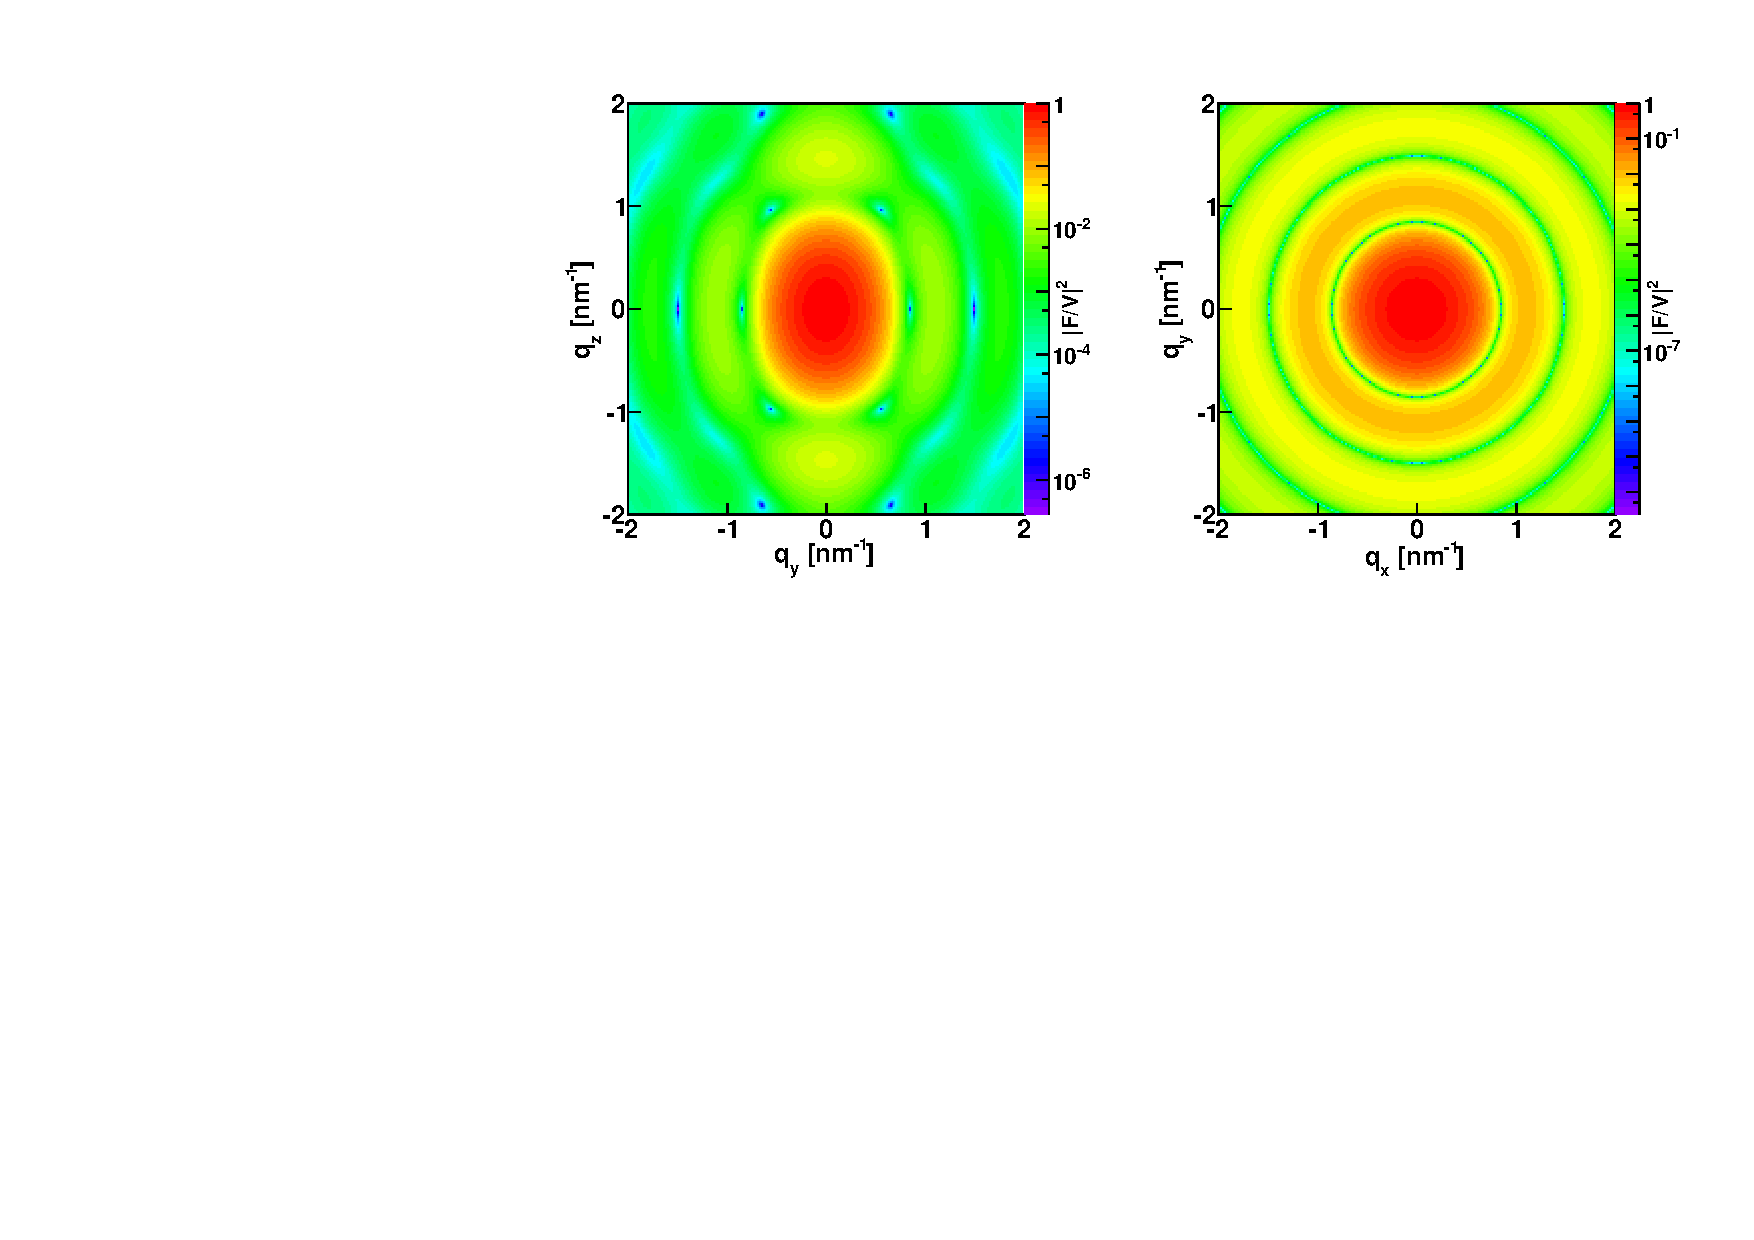
\includegraphics[width=0.9\textwidth]{Figures/figffsphere}
\end{center}
\caption{{\bf a:} $|F|^2$ plotted against $q_z$ and $q_y$, {\bf b:} $|F|^2$ plotted against $q_x$ and $q_y$, {\bf c:} slice of the picture {\bf a} along the $q_z$ axis, {\bf d:} slice of the picture {\bf b} along the $q_x$ axis.}
\end{figure}

\par


%\null\newpage

%\newpage{\pagestyle{empty}\cleardoublepage}
\newpage{\cleardoublepage}


\section{Formfactor Full Sphere}\SecLabel{FullSphere}
%\begin{lstlisting}[language=python, style=eclipseboxed,name=fffullsphere,nolol]
%from libBornAgainCore import * 
%fullsphere_ff = FormFactorFullSphere(5*nanometer)
%\end{lstlisting}
%\par
%~
%\par
Formfactor full sphere is represented as a sphere with radius $R$. 
\begin{figure}[ht]
\begin{center}
\includegraphics[width=0.6\columnwidth]{Figures/fullsphere}
\caption{Sketch of the formfactor full sphere. Left: front view, right: top view.}
\end{center}
\label{fullsphere}
\end{figure}

\begin{equation}
F(\mathbf q, R) = 4\pi R\times\frac{\sin(qR)-qR\cos(qR)}{(qR)^3}\times\exp\left(iq_zR\right)
\end{equation}

\begin{figure}[h]
\begin{center}
\includegraphics[width=0.9\textwidth]{Figures/figfffullsphere}
\end{center}
\caption{{\bf a:} $|F|^2$ plotted against $q_z$ and $q_y$, {\bf b:} $|F|^2$ plotted against $q_x$ and $q_y$, {\bf c:} slice of the picture {\bf a} along the $q_z$ axis, {\bf d:} slice of the picture {\bf b} along the $q_x$ axis.}
\end{figure}

\par

